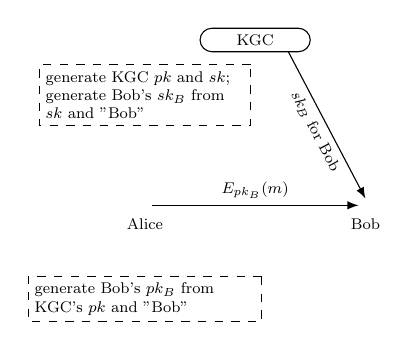
\begin{tikzpicture}[font=\footnotesize,scale=0.7, every node/.style={scale=0.7}]
\node (A) at (0,0) [label=below:Alice] {\Lisa};
\node (B) [right of = A, node distance = 4cm,label=below:Bob] {\Left\Bart};
\node (KGC) at (2,3) [rounded corners=1ex,minimum width=2cm,draw] {KGC};  
\node at (0,2) [text width=3.6cm, draw, dashed] {generate KGC $pk$ and $sk$; generate Bob's $sk_B$ from $sk$ and "Bob"};
\draw[-latex] (A) -- (B) node [midway,above] {$E_{pk_{B}}(m)$};
%\draw[-latex] (B.70) -- (KGC.350) node [sloped,midway,above] {I want to talk to Bob.};
\draw[-latex] (KGC.340) -- (B.90) node [sloped,midway,below] {$sk_{B}$ for Bob};
\node at (0,-1.7) [text width=4cm, draw, dashed] {generate Bob's $pk_{B}$ from KGC's $pk$ and "Bob"};
\end{tikzpicture}